% Original-research manuscript for IEEE Transactions on Aerospace and Electronic Systems.
% Build with pdfLaTeX, BibTeX, and two further pdfLaTeX passes in this directory.
\documentclass{IEEEtaes}
\usepackage{amsmath,amssymb,array,booktabs,graphicx,tikz}
\hypersetup{hidelinks,pdftitle={Single-Tag Range-Inertial Position Acquisition with Profiled Heading and a Rotating Bias Model},pdfauthor={},pdfsubject={Range-inertial navigation}}
\newcommand{\rz}{R_z}
\newcommand{\norm}[1]{\left\lVert#1\right\rVert}
\newcommand{\sk}[1]{[#1]_\times}
\newcommand{\trans}{^{\mathsf T}}
% IEEEtaes.bst prints note fields but does not display its entries' DOI metadata.
\newcommand{\articledoi}[1]{doi: \href{https://doi.org/#1}{\nolinkurl{#1}}}
\graphicspath{{figures/}}

% The official class inserts production fields before IEEE assigns a volume or issue.
% A running manuscript title and page number occupy the usual footer in this draft.
\makeatletter
\def\ps@manuscript{%
  \let\@oddhead\@empty\let\@evenhead\@empty
  \def\@oddfoot{\rffont Single-tag range--inertial position acquisition\hfil\thepage}%
  \def\@evenfoot{\rffont\thepage\hfil IEEE Transactions on Aerospace and Electronic Systems\enspace|\enspace Manuscript}}
\makeatother
\begin{document}
\title{Single-Tag Range--Inertial Position Acquisition with Profiled Heading and a Rotating Bias Model}
% Author names, affiliations and correspondence will be supplied by the authors.
\author{}
\pagestyle{manuscript}
% Suppress only the class's publisher-reserved first-page copyright footnote.
\let\manuscriptfootnotetext\footnotetext
\renewcommand{\footnotetext}[1]{}
\maketitle
\let\footnotetext\manuscriptfootnotetext
\thispagestyle{manuscript}

\begin{abstract}
An aircraft with a single ultra-wideband tag receives distances to different anchors at different times. Given gravity alignment, we use the intervening inertial motion to estimate the position at the latest sensor time with unknown heading and no vehicle thrust model. A squared-range relaxation supplies one heading candidate. A robust fit to the original distances then corrects the integrated trajectory for a body-fixed accelerometer offset. We derive when a free quadratic can represent the same correction and which part of the motion carries heading information. With the same candidate policy, motion correction and a trained radio mean reduce horizontal endpoint root-mean-square error from 1.625 to 0.159\,m on six indoor flights. Outdoors, motion correction alone reduces error from 2.930 to 1.631\,m against a prism reference on ten recordings. With common constant calibration, eight-anchor horizontal error is 0.133\,m, compared with 0.356\,m for a range-only quadratic reconstruction. The single heading candidate matches the objective reached with four uniform starts on all 528 indoor configurations within the prescribed tolerance, using 62.1\% fewer function evaluations. As a navigation application, conditional handoff to an invariant filter restores late horizontal tracking on all six indoor flights after a 20\,s outage.
\end{abstract}
\begin{IEEEkeywords}
Inertial navigation, invariant extended Kalman filter, observability, position acquisition, ultra-wideband ranging.
\end{IEEEkeywords}

\section{Introduction}\label{sec:intro}
A quadrotor emerging from radio shadow receives one range at a time. Each packet constrains the antenna to a sphere at the instant of the exchange. By the time another anchor replies, the aircraft has moved. Treating these ranges as a set of simultaneous spheres introduces a motion error. Integrating the inertial measurement unit (IMU) between exchanges links the antenna positions, but an error in tilt or accelerometer bias bends the integrated path. The bend grows with the age of the oldest packet. A longer window can therefore improve the geometry of multilateration while making the assumed inertial trajectory less accurate.

Published range-only methods recover a trajectory by imposing a basis on its positions~\cite{pacholska}, while a model of quadrotor thrust and drag supplies motion information to a moving-horizon tracker~\cite{pfeiffer}. We consider an alternative for an aircraft carrying one ultra-wideband (UWB) tag in a surveyed anchor field. Gravity alignment is available from an earlier IMU prefix. Absolute yaw and endpoint velocity are unknown. The desired output is the position at the most recent sensor time. Writing that fix into a running navigation filter poses a further question because velocity and attitude also determine the next predicted position.

Our formulation uses two pieces of information available to a single tag. The ranges locate the aircraft relative to the anchors, and the gravity-aligned IMU records the shape of its motion up to an unknown heading. In a squared-range relaxation, we eliminate the endpoint translation, velocity and auxiliary products analytically. The remaining unit-circle problem supplies a heading candidate for a single nonlinear fit to the original distances. Its global solution applies to the relaxed candidate objective.

The second contribution concerns how the measured shape should be corrected. We derive the endpoint displacement produced by a constant accelerometer offset rotating with the aircraft. It agrees to second order with a world-frame quadratic, then separates during a turn. A local information calculation identifies the yaw variation still visible after position, velocity and bias are refitted. Flight comparisons test the value of the inertial shape at matched packet times and the cost of choosing one heading candidate. A conditional handoff to an invariant extended Kalman filter (InEKF) tests whether the acquired motion restores tracking after an outage.

\section{Related work}\label{sec:related}
\subsection{Trajectory reconstruction and observability}
Batista \emph{et al.} obtained observability conditions and a filter for single-range navigation with measured relative velocity~\cite{batista}. Theodosis \emph{et al.} showed how quadratic outputs of certain linear systems admit a finite-dimensional linear immersion~\cite{theodosis}. Their single-anchor navigation example takes world acceleration as an input. Both results explain how motion supplies information missing from an instantaneous range. On a quadrotor, the accelerometer reports body-frame specific force. Converting it to world acceleration already requires the heading and bias that the window is asked to estimate.

Pacholska \emph{et al.} used an assumed trajectory basis to recover continuous position from distances alone~\cite{pacholska}. Lifting products of basis coefficients makes the algebra linear and leads to explicit recovery conditions. Goudar \emph{et al.} developed range-only trajectory initializers with guarantees under specified configurations of tags, beacons and motion~\cite{goudar}. A known baseline between body-mounted radios can supply attitude information that a single colocated tag lacks. Here, the known component is the trajectory shape obtained by integrating an IMU in a gravity-aligned frame. Separating the coefficients that enter linearly follows the variable-projection principle of Golub and Pereyra~\cite{varpro}. Our use of that principle leaves two coupled coefficients on a unit circle. The physically admissible raw-range trajectories form a smaller set than those admitted by the squared-range relaxation.

\subsection{Asynchronous fusion and inertial bias}
Tightly coupled UWB/IMU estimators directly relate the radio measurement to a moving pose. Hol \emph{et al.} connected heading estimation to acceleration excitation~\cite{hol}. Kok \emph{et al.} developed an optimization-based estimator with an asymmetric time-of-arrival error model~\cite{kok}. Li \emph{et al.} fitted continuous-time splines to asynchronous UWB and IMU samples~\cite{sfuise}. Jiang \emph{et al.} initialized a joint range--inertial graph and incrementally optimized it on recorded single-sided two-way ranging (TWR) data~\cite{jiang}. Incremental smoothing can efficiently relinearize a trajectory as new factors arrive~\cite{isam2}. These methods represent motion throughout a trajectory. Our window compresses the translational uncertainty into endpoint position, endpoint velocity and three acceleration-correction coefficients. This makes it possible to compare two physical explanations for the same range history at equal model dimension.

IMU preintegration incorporates the sensitivity of integrated increments to sensor biases~\cite{forster}. We use that sensitivity in an endpoint-centered form. It has two consequences for acquisition. The leading position perturbation can agree with a constant world acceleration even when the true offset is body-fixed. With strong rotation, an unrestricted world acceleration and a constant body bias produce different families of positions. The heading question is consequently about which component of a change in yaw survives after fitting all the motion coefficients.

\subsection{Radio calibration and navigation benchmarks}
Radio error also varies systematically with geometry and hardware. Prorok and Martinoli learned spatial error models for indoor ranging~\cite{prorok}. Ledergerber and D'Andrea used maximum likelihood to calibrate systematic ranging errors~\cite{ledergerber}. Shalaby \emph{et al.} characterized antenna delays and power-dependent bias and variance in TWR~\cite{shalaby}. Zhao \emph{et al.} combined learned bias correction with robust filtering for time differences of arrival (TDoA)~\cite{zhao}. Goudar and Schoellig studied excitation conditions for estimating the spatial and temporal offsets between a radio and an IMU~\cite{goudarcal}. Ferrero-Guill\'en \emph{et al.} analyzed a further source of error arising from motion during the messages of an asynchronous TWR exchange~\cite{motiontwr}. Evaluating a finished range at its transaction time addresses motion \emph{between} packets. It leaves motion within the exchange and unmeasured antenna delays in the observation error. We therefore compare motion models under a common radio calibration and examine transfer with its coefficients removed.

Pfeiffer \emph{et al.} released a vehicle-model moving horizon estimator (MHE), a companion extended Kalman filter (EKF) and a quadrotor dataset~\cite{pfeiffer,delftdata}. Their later MHE uses adaptive step sizes and switching variables for outlier handling~\cite{pfeiffer25}. We test the released 2021 classes at matched endpoint times and retain their dynamics and attitude handling. Oursland and Mehrabian~\cite{oursland} used an InEKF for a tag with a known lever arm and signed TDoA. Invariant error coordinates can improve the linearization of navigation dynamics under the hypotheses studied by Barrau and Bonnabel~\cite{barrau}. They cannot supply an independent heading measurement. We use the native TDoA filter on recordings with measured attitude, and assess the zero-lever-arm TWR acquisition model on separate flights.

Table~\ref{tab:landscape} relates each method's motion input to its output. We compare position at the last packet available to every estimator.

\begin{table*}[t]
\centering\caption{Motion assumptions and estimation targets in related range-based navigation methods.}
\label{tab:landscape}\tablefont
\begin{tabular*}{\textwidth}{@{\extracolsep{\fill}}>{\raggedright\arraybackslash}p{.26\textwidth}>{\raggedright\arraybackslash}p{.34\textwidth}>{\raggedright\arraybackslash}p{.33\textwidth}@{}}
\toprule
Approach&Motion information&Estimation target\\\midrule
Range-only lifting~\cite{pacholska}&Assumed finite trajectory basis&Continuous single-tag position\\
Range-only initialization~\cite{goudar}&Rigid tag geometry and a prescribed motion model&Pose or trajectory under tag and beacon geometry conditions\\
UWB--inertial smoothing~\cite{sfuise,jiang}&IMU samples with a spline or factor graph&Trajectory and inertial states over the window\\
Quadrotor MHE and EKF~\cite{pfeiffer,pfeiffer25}&Vehicle-specific thrust and drag models&Rolling or recursive position and velocity\\
TDoA InEKF~\cite{oursland}&IMU propagation and an antenna lever arm&Recursive attitude, velocity and position\\
Single-tag acquisition (this work)&Measured inertial shape and a rotating body-fixed offset&Endpoint position and velocity with unknown initial heading\\
\bottomrule
\end{tabular*}
\end{table*}

\section{A yaw candidate from asynchronous ranges}\label{sec:profile}
\subsection{Endpoint coordinates}
Let \(R\) map body vectors to a navigation frame with vertical \(e_3\), and write \(v,p\) for the velocity and position of the IMU. The accelerometer and gyro report \(f_m,\omega_m\) with biases \(b_a,b_g\). For nominal propagation,
\begin{equation}
 \dot R=R\sk{\omega_m-b_g},\quad
 \dot v=R(f_m-b_a)+g,\quad \dot p=v ,
 \label{eq:ins}
\end{equation}
where \(g=-9.81e_3\) in m/s\(^2\) and \(\sk{x}y=x\times y\). A TWR transaction \(i\) supplies range \(z_i\) to surveyed anchor \(a_i\) at time \(t_i\). The window takes the antenna and IMU to be colocated. With \(D_i=\norm{p_i-a_i}\) and \(n_i=(p_i-a_i)/D_i\), its observation model is
\begin{equation}
 z_i=D_i+\mu_{a_i}(D_i,n_i)+e_i . \label{eq:observation}
\end{equation}
Here the anchor subscript on \(\mu\) identifies a radio link. The scale \(\sigma_i\) describes the inlier range error. The fit also accommodates occasional large residuals.

Write \(R(t)=\rz(\psi)Q(t)\), where \(Q\) follows nominal gravity alignment and gyro integration in an arbitrary initial yaw frame. Let \(s(t)\) be a nominal double integral of acceleration in that frame and set \(T\) to the last available sample. Defining \(\tau_i=t_i-T\) gives
\begin{align}
 d_i &= s(t_i)-s(T)-\tau_i\dot s(T),\nonumber\\
 p_i &= p_T+\tau_i v_T+\rz(\psi)d_i . \label{eq:affine}
\end{align}
Reanchoring removes the integration constants even when the starting velocity is unknown. Both \(d(T)\) and \(\dot d(T)\) vanish. Gravity commutes with the yaw rotation, so \(d_i\) includes its displacement. The design evaluates the held IMU model at each transaction time. No simultaneous group of anchor readings is required. We call \eqref{eq:affine} the \emph{affine} model because its free translation is affine in time. Its nominal inertial path can be highly curved.

\subsection{Lifting and elimination of translation}
For the seed, write \(p_i=c(\tau_i)+\rz(\psi)d_i\), where \(c(\tau)=\sum_{j=0}^{K}c_j\tau^j\). Acquisition uses \(K=1\). The general degree clarifies what information a more flexible translation removes. Subtract a constant radio offset to obtain \(r_i=z_i-\beta_{a_i}\) (zero offset when uncalibrated), and form
\begin{equation}
 y_i=\tfrac12(r_i^2-\sigma_i^2-\norm{a_i}^2-\norm{d_i}^2)
              +a_{iz}d_{iz}. \label{eq:y}
\end{equation}
In the noiseless identity take \(\sigma_i=0\). For \(u=(\cos\psi,\sin\psi)\trans\), expansion then yields
\begin{equation}
 y=B\nu+Dc+Cu . \label{eq:lift}
\end{equation}
The vector \(c\) stacks the \(c_j\). The row of \(B\) contains \(\tau_i^\ell\) for \(0\le\ell\le 2K\), followed by the pairs \((\tau_i^j d_{ix},\tau_i^j d_{iy})\) for \(0\le j\le K\). The remaining rows are
\begin{align}
 D_{ij}&=\tau_i^j[-a_{ix},-a_{iy},d_{iz}-a_{iz}],\nonumber\\
 C_i&=[-a_{ix}d_{ix}-a_{iy}d_{iy},\ a_{ix}d_{iy}-a_{iy}d_{ix}].
 \label{eq:rows}
\end{align}
For a physical path, the coefficients in \(\nu\) are constrained. The coefficient of \(\tau^\ell\) in \(\norm{c(\tau)}^2/2\) is \(\tfrac12\sum_{j+k=\ell} c_j\trans c_k\). The two horizontal cross-term coefficients for each \(j\) are the components of \((\rz(\psi)\trans c_j)_{xy}\). Releasing these identities makes \(\nu\) independent of \(c\) and \(u\). This is the only relaxation in \eqref{eq:lift}.

For an ideal zero-mean Gaussian inlier, the centered half-squared range has variance \(D_i^2\sigma_i^2+\sigma_i^4/2\). We substitute \(\max(r_i,\sigma_i)\) for the unknown distance in this expression and place the inverse standard deviations on the diagonal of \(W\). With \(L=W[B\ D]\), define \(P=I-LL^\dagger\), \(\bar y=PWy\) and \(\bar C=PWC\). Minimizing over all the linear coefficients gives
\begin{equation}
 F(\psi)=\norm{\bar y-\bar C u(\psi)}^2. \label{eq:circle}
\end{equation}
This projection is exact within the relaxed squared-range model at fixed weights. The implementation removes the left singular vectors whose singular values exceed \(10^{-10}\) times the largest value. It never needs to materialize the dense projector.

Set \(H=\bar C\trans\bar C,\ h=\bar C\trans\bar y\) and \(\Delta=H_{22}-H_{11}\). The terms varying with yaw are
\begin{align}
 F(\psi)={}&-\tfrac{\Delta}{2}\cos2\psi+H_{12}\sin2\psi \nonumber\\
           &-2h_1\cos\psi-2h_2\sin\psi+\mathrm{const}. \label{eq:harmonic}
\end{align}
Only the first two angular harmonics remain. With \(q=\tan(\psi/2)\), setting the derivative to zero gives
\begin{align}
 0={}&(H_{12}+h_2)q^4+2(h_1-\Delta)q^3-6H_{12}q^2 \nonumber\\
     &+2(h_1+\Delta)q+(H_{12}-h_2). \label{eq:quartic}
\end{align}
Checking the real roots and \(\psi=\pi\) covers the circle. The implementation also checks zero for a degenerate polynomial. We call the policy that retains one minimum of \eqref{eq:circle} \emph{Profile-1}. Its global solution concerns the seed objective. The subsequent robust distance fit can have distinct local minima.

\subsection{Identifiability and sensitivity of the heading seed}
For an exact noiseless model the physical \(u_\star\) makes \eqref{eq:circle} zero. If \(\bar C\) has column rank two, every minimizer obeys \(\bar C(u-u_\star)=0\) and hence equals \(u_\star\). Once yaw is known, translation in the lifted equations is unique if \((I-WB(WB)^\dagger)WD\) has rank \(3(K+1)\). These are sufficient conditions. A rank-one projected system may intersect the circle twice, or tangentially at one point.

The row count gives a practical interpretation. For \(K=1\) the lift has seven auxiliary and six translation columns. If these 13 columns are independent, at least 15 transactions are needed to leave two projected directions. Adding a quadratic raises these counts to 11 and nine, hence 22 transactions in general position. Collecting that many packets does not guarantee useful geometry. Poor anchor height diversity or a nearly polynomial inertial shape can leave the smallest singular value of \(\bar C\) very small. Even perfect arithmetic on \eqref{eq:quartic} then gives little protection against an error in \(d_i\).

There is also a finite perturbation bound. At fixed design let \(\bar y=\bar C u_\star+\epsilon\), and let \(\hat u\) minimize \eqref{eq:circle}. Feasibility of \(u_\star\) gives \(\|\bar y-\bar C\hat u\|\le\|\epsilon\|\). The triangle inequality and the chord length on the unit circle then yield
\begin{equation}
 \left|\sin\frac{\hat\psi-\psi_\star}{2}\right|
 \le \frac{\norm{\epsilon}}{\sigma_{\min}(\bar C)}
 \quad\text{if }\operatorname{rank}(\bar C)=2 .
 \label{eq:chord}
\end{equation}
The denominator can be computed before any nonlinear fit. The numerator is the departure from the physical heading in the projected equations, which can include inertial mismatch. This relation explains why concentrating the anchors in a shallow plane and adding more starts address different sources of error.

\section{Fitting the physical trajectory}\label{sec:fit}
\subsection{A rotating accelerometer offset}
Suppose the true accelerometer bias differs from the nominal value by a constant \(\delta b\) over the window. At fixed nominal rotation its contribution to world acceleration is \(-\rz(\psi)Q(t)\delta b\). Integrating twice and subtracting the endpoint position and velocity contributions gives
\begin{align}
 B_i^a &= \int_{t_i}^{T}(s-t_i)Q(s)\,ds,\label{eq:bint}\\
 p_i &=p_T+\tau_i v_T+\rz(\psi)(d_i-B_i^a\delta b).
 \label{eq:bias}
\end{align}
The sign of the kernel follows from integrating backward from \(T\) with zero terminal displacement and velocity. The integration in \eqref{eq:bint} is exact for the held rotation samples in the estimator. A changing gyro bias or an incorrect tilt changes the nominal rotation itself and can produce errors outside this three-parameter family. We interpret the fitted coefficient as a short-window motion correction.

On flights with independent radio calibration data we use the mean
\begin{equation}
 \mu_a(D,n)=\beta_a^{\,g}+s_a(D-\bar D_a)+\kappa_a\trans n .
 \label{eq:mean}
\end{equation}
The link intercept, slope and direction coefficients are robust ridge estimates from training flights. The simpler constant-offset model uses a training median \(\beta_a\). Both use the same training median-absolute-deviation range scales. A line-of-sight coefficient can absorb an apparent anchor displacement, since a small displacement \(\delta a\) changes distance by \(-n\trans\delta a\) to first order. Its presence in \eqref{eq:mean} therefore does not identify a physical survey error. We freeze these coefficients before scoring and remove the whole mean at a site without calibration.

Define \(r_i^{\,p}=(D_i+\mu_{a_i}-z_i)/\sigma_i\), and let \(\rho_2(r)\) equal \(r^2/2\) for \(|r|\le2\) and \(2|r|-2\) otherwise. The endpoint fit minimizes
\begin{equation}
 \min_{p_T,v_T,\psi,\delta b}\ \sum_i\rho_2(r_i^{\,p})+\frac{\norm{\delta b}^2}{2\sigma_b^2},
 \qquad \sigma_b=0.10\ {\rm m/s^2}. \label{eq:raw}
\end{equation}
The prior on the three bias components stays quadratic. We first fit a constant-velocity translation to the ranges from two starts, a squared-range linear solution and a stationary anchor-centroid start. Only the better translation enters \eqref{eq:raw}. Profile-1 supplies its yaw and \(\delta b\) starts at zero. Thus the principal acquisition method performs two common translation fits and one final ten-variable distance fit. The raw fit has a cap of 120 function evaluations per start. The affine control follows the same seed policy with \(\delta b=0\).

Differentiating the radio mean matters when the aircraft crosses a learned direction gradient. Write \(\ell_i=\rz(\psi)(d_i-B_i^a\delta b)\). The two factors of the residual Jacobian are
\begin{align}
 g_i &= (1+s_a)n_i+(I-n_i n_i\trans)\kappa_a/D_i,\nonumber\\
 G_i &= [\,I,\ \tau_i I,\ e_3\times\ell_i,\ -\rz(\psi)B_i^a\,],\nonumber\\
 J_i &= \sigma_i^{-1} g_i\trans G_i . \label{eq:jac}
\end{align}
For the constant radio mean \(g_i=n_i\). The second term of \(g_i\) acts perpendicular to the line of sight and accounts for the change in predicted direction when the fitted position moves.

\subsection{Local equivalence to a quadratic correction}
Let \(h_i=T-t_i\). A freely fitted world acceleration \(c_W\) adds \(\tfrac12 h_i^2 c_W\) to \eqref{eq:affine}. It costs three parameters, the same number as \(\delta b\), and has no prior. For a fixed attitude the two motion models span exactly the same corrections through \(c_W=-\rz(\psi)Q(T)\delta b\). When \(\|\dot Q\|_2\le\Omega\), the difference between their leading terms obeys
\begin{equation}
 \big\| B_i^a-\tfrac12 h_i^2 Q(T)\big\|_2
 \le \int_0^{h_i}(h_i-u)\Omega u\,du
 =\tfrac16\Omega h_i^3 . \label{eq:bound}
\end{equation}
If \(Q\) is twice continuously differentiable, expanding \eqref{eq:bint} gives \(B_i^a=\tfrac12h_i^2 Q(T)-\tfrac16h_i^3\dot Q(T)+O(h_i^4)\). Rotation first changes the shape at cubic order. In Fig.~\ref{fig:turn}, the two displacement corrections differ by 0.078 m at 2 s and 0.575 m at 4 s. A short or weakly turning segment can benefit from correcting acceleration before it distinguishes the two models.

\begin{figure}[t]
\centering
% Analytic bias-versus-quadratic displacement in a constant-rate planar turn.
% The curves are evaluated directly from the continuous integral in the text.
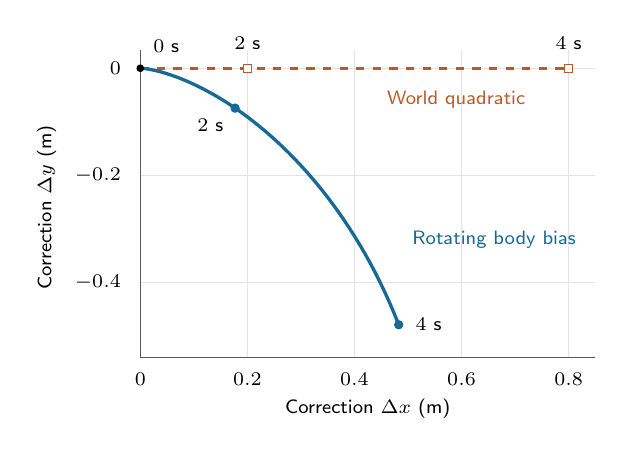
\begin{tikzpicture}[x=6.8cm,y=6.8cm,font=\sffamily\scriptsize]
  \definecolor{quadraticcolor}{RGB}{183,91,40}
  \definecolor{bodycolor}{RGB}{23,106,148}
  % Equal metric scales: these are correction displacements, not aircraft paths.
  \foreach \x in {0,.2,.4,.6,.8}{
    \draw[gray!22] (\x,-.54)--(\x,.035);
    \node[anchor=north] at (\x,-.55) {\pgfmathprintnumber[fixed,precision=1]{\x}};
  }
  \foreach \y in {-.4,-.2,0}{
    \draw[gray!22] (0,\y)--(.85,\y);
    \node[anchor=east] at (-.018,\y) {\pgfmathprintnumber[fixed,precision=1]{\y}};
  }
  \draw[black!65] (0,.035)--(0,-.54)--(.85,-.54);
  \node[rotate=90] at (-.175,-.26) {Correction $\Delta y$ (m)};
  \node[anchor=north] at (.425,-.60) {Correction $\Delta x$ (m)};
  % Endpoint acceleration is +0.10 e_x m/s^2; omega=0.60 rad/s and h=T-t.
  % q_W=a h^2 e_x/2; q_B=a[(1-cos(omega h)),sin(omega h)-omega h]/omega^2.
  \draw[quadraticcolor,very thick,dashed] (0,0)--(.8,0);
  \draw[bodycolor,very thick,domain=0:4,samples=90,variable=\h]
    plot ({.1*(1-cos(deg(.6*\h)))/.36},{.1*(sin(deg(.6*\h))-.6*\h)/.36});
  \fill[black] (0,0) circle[radius=1.4pt];
  \node[anchor=south west] at (.006,.012) {$0$ s};
  \foreach \x/\label in {.2/2,.8/4}{
    \node[draw=quadraticcolor,fill=white,inner sep=0pt,minimum size=3pt] at (\x,0) {};
    \node[anchor=south] at (\x,.017) {$\label$ s};
  }
  \fill[bodycolor] (.177123,-.074434) circle[radius=1.7pt];
  \node[anchor=north east] at (.173,-.077) {$2$ s};
  \fill[bodycolor] (.482609,-.479038) circle[radius=1.7pt];
  \node[anchor=west] at (.496,-.479) {$4$ s};
  % Direct labels and distinct marker/line styles retain monochrome legibility.
  \node[quadraticcolor,anchor=north] at (.59,-.025) {World quadratic};
  \node[bodycolor,anchor=west] at (.49,-.32) {Rotating body bias};
\end{tikzpicture}

\caption{Displacement corrections in an analytic planar turn. Both start with the same terminal correction acceleration \(+0.10e_x\) m/s\(^2\). At a yaw rate of 0.60 rad/s the body-fixed correction curves away from the world-frame quadratic. Markers give time before the endpoint. Both axes have the same spatial scale.}
\label{fig:turn}
\end{figure}

\subsection{Heading sensitivity after fitting nuisance states}
For local analysis, multiply each radio Jacobian row in \eqref{eq:jac} by \(\sqrt{\min(1,2/|r_i^{\,p}|)}\), taking weight one at zero. Partition the result into the yaw column \(\tilde j_\psi\) and the position, velocity and correction columns \(\tilde J_n\). To first order, the part of a yaw change that these nuisance variables cannot absorb has squared norm
\begin{equation}
 \mathcal I_{\psi\mid n}
 =\min_a\norm{\tilde j_\psi-\tilde J_n a}^2
 =\norm{(I-\tilde J_n\tilde J_n^\dagger)\tilde j_\psi}^2 .
 \label{eq:curvature}
\end{equation}
This is a local Gauss--Newton curvature with fixed robust weights. Adding the bias prior penalizes the minimizing nuisance motion and can increase this number without adding information from the ranges. A locally sharp minimum can also coexist with a distant yaw mode.

A limiting case exhibits exact ambiguity. Assume constant \(Q\), constant measured specific force \(f_m\), zero lever arm and a freely fitted constant bias. For any second yaw \(\psi'\), choose
\begin{equation}
 b_a'=f_m-Q\trans\rz(\psi')\trans\rz(\psi)Q(f_m-b_a).
 \label{eq:gauge}
\end{equation}
Both pairs \((\psi,b_a)\) and \((\psi',b_a')\) generate the same world acceleration. With the same starting position and velocity, their positions, radio directions and all ranges coincide even for ideal anchors. A bias prior can select between them. The radio data cannot. A time-varying \(f_m\) generally makes the right side of \eqref{eq:gauge} time dependent, so constant attitude alone is insufficient for this ambiguity.

A related loss occurs with free polynomial translation. Adding a vector polynomial \(b(\tau)\) of degree at most \(K\) to \(d\) and replacing \(c(\tau)\) by \(c(\tau)-\rz(\psi)b(\tau)\) preserves every position for each fixed yaw. If \(d\) lies entirely in this polynomial space, varying yaw cannot change the best range fit. The bias model in \eqref{eq:raw} restricts its allowed correction through \(B_i^a\) and a prior.

\section{Flight data and comparison protocol}\label{sec:protocol}
\subsection{Acquisition windows and reference positions}
The Delft dataset~\cite{delftdata} contains two TWR recordings for each of six motions. We use the earlier recording of each motion to fit radio calibration and the later one to score acquisition. All six evaluation flights share the room and campaign date and were available during method development. A held-motion calibration control excludes the earlier recording of the target motion as well. It tests whether a directional calibration generalizes to a different motion in the same anchor installation.

The replay clock starts after a 1.5\,s IMU prefix for tilt and nominal bias. An offline 0.20\,s offset aligns OptiTrack for scoring at the actual last sample of each window. Reference positions select the supported interval and are withheld from the estimator. We test 2 and 4 s windows ending at 5, 10, 20 and 30 s, adding 8 s windows at the last three times. The six flights yield 66 physical windows and 24 distinct endpoint times. Testing all eight anchors and the four lowest gives 132 layout-specific windows.

For the seed comparison we also solve in four equivalent inertial yaw coordinate frames. The geometry and data are unchanged, although a finite-budget optimizer can reach different minima. The 528 fits characterize solver behavior across coordinates. We additionally fix one coordinate frame when comparing flights so that a flight with more yaw parameterizations receives no extra evidential weight.

The outdoor QDrone dataset~\cite{qdrone} contributes ten recordings from a field, a building, a bridge and a tunnel. Nested 2, 4 and 8\,s windows end at the midpoint of sensor coverage in each recording, giving 30 segments at ten endpoint instants. The published total-station prism position serves as a proxy because its exact transform to the antenna is unavailable. Both fits use the same IMU prefix, zero radio mean and a \(0.30\) m radio scale. We use the registered coordinates directly, without site-specific radio fitting or truth-based realignment.

\subsection{Metrics and matched inputs}
For window \(i\), let \(e_{i,xy}=\norm{\hat p_{i,xy}-p^*_{i,xy}}\). For an explicitly specified set \(S\) we report
\begin{equation}
 E_{xy}(S)=\sqrt{|S|^{-1}\sum_{i\in S}e_{i,xy}^2}. \label{eq:score}
\end{equation}
Vertical (\(Z\)) and three-dimensional (3D) errors use the corresponding components of the position residual. Within the same set \(E_{\rm 3D}^2=E_{xy}^2+E_z^2\), which allows a vertical failure to be distinguished from a horizontal one. We use flight-level pairs to show heterogeneity and retain the larger set of fits where measuring optimization reliability is the purpose. The reported summaries are descriptive. Overlapping windows are correlated, as are alternative layouts of the same anchor field.

For each Delft comparison, the estimators restart at the same window boundary and receive the same positive range updates and anchor coordinates. We supply either raw ranges with a 0.25 m scale or training-corrected constant offsets and scales. The released MHE uses 20 internal nodes at 50 Hz, one gradient step and sample-consensus rejection. Its gradient ignores the supplied variances. The released EKF runs at 100 Hz. Both retain the authors' zero translation, level zero-yaw attitude and thrust/drag model with an acceleration-based thrust proxy. We disable auxiliary height and consume pending final packets. Our method uses the IMU prefix for tilt and searches yaw.

For continuous tracking we compute a time-domain XY RMSE from the most recently emitted state on a 20 Hz grid within each flight and interval. Section~\ref{sec:handoff} reports medians over reference-supported flights and paired differences between policies.

\section{Endpoint accuracy and competing estimators}\label{sec:results}
\subsection{Effects of trajectory correction and radio calibration}
Table~\ref{tab:endpoints} compares the affine and bias-corrected fits under the same single-candidate policy. In Delft the headline comparison changes both the motion correction and the radio mean. In QDrone the mean is zero for both fits. Separating the two changes is essential, since both can reduce a systematic range residual.

\begin{table}[t]
\caption{Endpoint RMSE in metres with one profiled yaw candidate per fit. Delft pools all four yaw coordinates. QDrone uses the prism proxy.}
\label{tab:endpoints}\centering\tablefont
\setlength{\tabcolsep}{4pt}
\begin{tabular}{@{}lrrrcrrr@{}}
\toprule
&\multicolumn{3}{c}{Affine}& &\multicolumn{3}{c}{Body bias}\\
\cmidrule(lr){2-4}\cmidrule(l){6-8}
Population&XY&\(Z\)&3D&&XY&\(Z\)&3D\\\midrule
Delft, eight&1.585&.758&1.757&&.116&.209&.239\\
Delft, low four&1.664&1.163&2.030&&.192&.526&.560\\
Delft, pooled&1.625&.981&1.898&&.159&.400&.431\\
QDrone&2.930&1.655&3.365&&1.631&1.779&2.414\\
\bottomrule
\end{tabular}
\end{table}

\begin{figure*}[t]
\centering
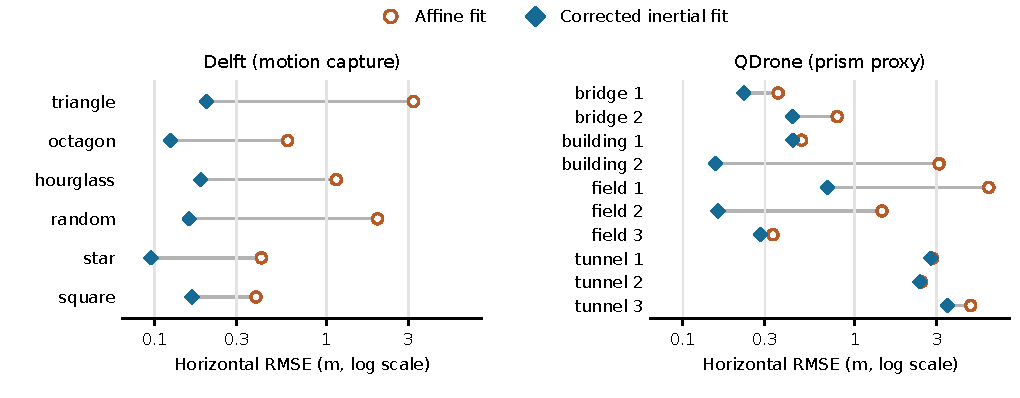
\includegraphics[width=\textwidth]{flight_endpoints.pdf}
\caption{Horizontal endpoint RMSE by recording. Each line joins an affine fit to a corrected inertial fit at the same endpoints. Delft includes 22 errors per flight at one yaw coordinate and adds a trained radio mean to the correction. QDrone pools three windows per recording and changes only the motion model. The horizontal axis is logarithmic.}
\label{fig:endpoints}
\end{figure*}

Across Delft configurations, horizontal RMSE falls by 90.2\%. The correction improves 440 of 528 paired errors, including all 144 configurations with an 8 s window. At 2, 4 and 8 s, pooled XY changes from \(0.222,\ 0.709,\ 2.991\) m to \(0.164,\ 0.175,\ 0.126\) m. With the yaw coordinate fixed, all six flights improve (Fig.~\ref{fig:endpoints}) and pooled XY falls from 1.645 to 0.159 m.

On QDrone, motion correction reduces pooled horizontal error to the registered prism by 44.3\% without site calibration. The 2, 4 and 8 s values change from \(1.634,\ 2.120,\ 4.312\) m to \(1.659,\ 1.629,\ 1.605\) m. Pooling the three lengths gives an improvement in every recording.

\begin{table}[t]
\caption{Delft control for motion and radio calibration. Four uniform yaw starts, reference coordinate and 66 physical windows per layout. Entries are RMSE in metres.}
\label{tab:motion}\centering\tablefont
\begin{tabular}{@{}lcrrrr@{}}
\toprule
& &\multicolumn{2}{c}{Eight anchors}&\multicolumn{2}{c}{Low four}\\
\cmidrule(lr){3-4}\cmidrule(l){5-6}
Motion&Radio&XY&3D&XY&3D\\\midrule
Affine&Constant&1.631&1.799&1.665&2.029\\
Quadratic&Constant&.127&.320&.201&.924\\
Body bias&Constant&.133&.279&.203&.874\\
Affine&Directional&1.654&1.756&1.653&1.924\\
Quadratic&Directional&.111&.273&.188&.591\\
Body bias&Directional&.116&.239&.192&.560\\
\bottomrule
\end{tabular}
\end{table}

With four starts held fixed (Table~\ref{tab:motion}), the affine fit exceeds 1.6 m in XY under both radio models. Either three-parameter motion correction removes most of that error. Under directional calibration the world quadratic and body bias give 0.155 and 0.159 m in pooled XY, winning three flights each. Their 3D errors are 0.460 and 0.431 m. These results agree with the leading-order equivalence in \eqref{eq:bound}. On QDrone the corresponding XY errors are 1.677 and 1.631 m.

Calibration adds a benefit that survives holding out the target motion from training. Changing the body-model mean from constant to directional changes XY from 0.135 to 0.119 m with eight anchors and from 0.204 to 0.199 m with the four lowest. The corresponding 3D changes are 0.289 to 0.250 m and 0.864 to 0.616 m. The larger 3D gain with low anchors reflects the sensitivity of height to the range mean.

\subsection{Cost and reliability of the yaw candidate}
We next fix the body model and compare its observed objective for a local yaw, Profile-1 and four uniform yaw starts. Let \(J\) denote the stored objective in twice the normalization of \eqref{eq:raw}. A miss on a real window means \(J-J_{\min}>10^{-4}(1+J_{\min})\), where \(J_{\min}\) is the best among these three policies for that same window. Raw objectives across different motion families have different meanings and are never used for this count.

\begin{table}[t]
\caption{Delft seed policies on the same 528 configurations and body-bias objective. Evaluations include both common translation fits. Capped final solutions are retained.}
\label{tab:seed}\centering\tablefont
\begin{tabular}{@{}lrrrr@{}}
\toprule
Yaw policy&Misses&Evaluations&XY (m)&3D (m)\\\midrule
One local yaw&7&36,313&.154&.429\\
Profile-1&0&32,789&.159&.431\\
Four uniform yaws&0&86,508&.159&.431\\\bottomrule
\end{tabular}
\end{table}

Profile-1 reaches the best observed objective within tolerance everywhere in Table~\ref{tab:seed}, using 62.1\% fewer function evaluations than four starts. A single local yaw misses seven times despite giving similar physical endpoint errors. On the outdoor recordings the miss counts for local, profiled and four-start fits are 1, 0 and 0. Switching the Delft Profile-1 \emph{motion model} from affine to body bias uses 32,632 versus 32,789 evaluations, an increase of 0.48\%. The evaluation count includes both translation fits. Per-evaluation work varies with the number of fitted variables.

A simulation tests the affine-model seed 30 m horizontally from the centroid of eight anchors at \((\pm4,\pm4,z)\) m, \(z\in\{0,h\}\). Each of 200 windows per geometry contains 4 s of inertial motion and 240 ranges with 0.10 m Gaussian noise. Success is within \(\max(10^{-3},10^{-5}|J_{\min}|)\) of the best of five policies (local, Profile-1 and 2, 4 or 12 uniform starts). At \(h=3\) m, Profile-1 and two starts both have zero misses and 0.509 m 95th-percentile 3D error. Their median times are 47.1 and 66.6 ms in 40 serial trials per policy on an i5-12600KF with single-threaded BLAS. At \(h=0.1\) m they miss 12 and 10 times, respectively. Shallow geometry also raises the Profile-1 95th-percentile 3D error to 3.946 m.

\subsection{Range-only and vehicle-model estimators}
The relaxation of Pacholska \emph{et al.}~\cite{pacholska} reconstructs motion using only the ranges. We evaluate the published line basis \((1,t)\) and a prespecified quadratic \((1,t,t^2)\) in the same solver. The latter represents the entire path, whereas the quadratic in Table~\ref{tab:motion} corrects a measured inertial path. Under common constant calibration, incorporating the IMU and fitting the body offset reduces horizontal RMSE from 0.356 to 0.133 m with eight anchors and from 0.474 to 0.204 m with the four lowest (Table~\ref{tab:published}). On the low layout the corresponding vertical errors are 7.982 and 0.854 m. The range-only linear system has full numerical rank in every window. The inertial shape supplies additional structure when shallow sight lines carry little independent height information.

\begin{table*}[t]
\centering
\caption{Published-method endpoint comparison on Delft. Each entry is an RMSE in metres over 66 windows per layout. Constant and raw rows are separate shared-input comparisons. The single Profile-1 row uses the body model.}
\label{tab:published}\tablefont
\begin{tabular}{@{}llrrrrrr@{}}
\toprule
& &\multicolumn{3}{c}{Eight anchors}&\multicolumn{3}{c}{Four lowest anchors}\\
\cmidrule(lr){3-5}\cmidrule(l){6-8}
Estimator and configuration&Radio&XY&\(Z\)&3D&XY&\(Z\)&3D\\\midrule
Pacholska \emph{et al.}, degree one, unweighted&Constant&.669&.425&.793&.689&5.803&5.844\\
Pacholska \emph{et al.}, degree one, author weights&Constant&.672&.411&.788&.676&6.268&6.305\\
Range-only degree two, author weights&Constant&.356&.491&.606&.474&7.982&7.996\\
Pfeiffer \emph{et al.}, author MHE&Constant&.121&.321&.343&.187&.876&.895\\
Pfeiffer \emph{et al.}, author EKF&Constant&.105&.231&.254&.188&.869&.889\\
Single Profile-1 with body bias&Constant&.133&.245&.279&.204&.854&.878\\\midrule
Pfeiffer \emph{et al.}, author MHE&Raw&.150&.549&.569&.219&.235&.321\\
Pfeiffer \emph{et al.}, author EKF&Raw&.172&.506&.534&.229&.243&.334\\
Single Profile-1 with body bias&Raw&.205&.523&.562&.397&.241&.465\\
\bottomrule
\end{tabular}
\end{table*}

\begin{figure*}[t]
\centering
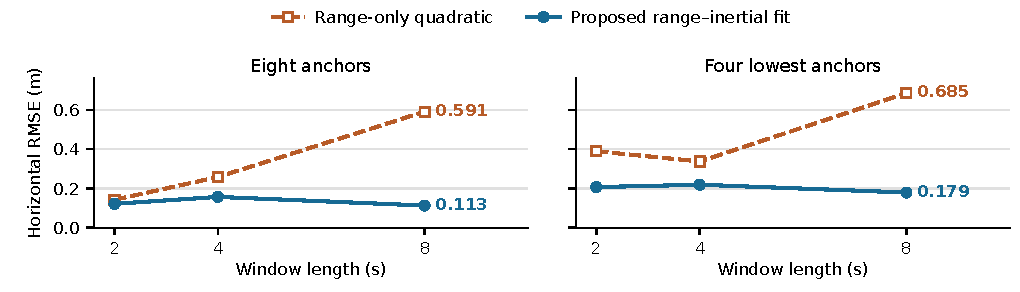
\includegraphics[width=\textwidth]{window_length_comparison.pdf}
\caption{Effect of measured inertial shape on horizontal endpoint RMSE. The quadratic range-only reconstruction and proposed fit share the range packets, constant calibration and endpoints. Each layout supplies 24, 24 and 18 windows at 2, 4 and 8 s. Both panels use the same linear scale. Table~\ref{tab:published} includes the vehicle-model EKF and MHE.}
\label{fig:length}
\end{figure*}

Fig.~\ref{fig:length} shows where the improvement occurs. On the eight-anchor layout, the horizontal error of the range-only quadratic rises from 0.142 m at 2 s to 0.591 m at 8 s. The inertial fit gives 0.121 and 0.113 m at those durations. With the four lowest anchors the corresponding 8 s errors are 0.685 and 0.179 m. The additional IMU input allows longer segments to retain measured turns, while a range-only polynomial must explain the entire maneuver using the same few coefficients.

With eight anchors and constant correction, the proposed method reaches 0.279 m in 3D, between the vehicle-model EKF (0.254 m) and MHE (0.343 m) of Pfeiffer \emph{et al.}~\cite{pfeiffer}. The respective counts within 0.5 m are 63, 65 and 56 of 66. Both vehicle estimators achieve lower pooled XY. The single-tag window reaches comparable 3D accuracy with free yaw and without thrust, mass or drag parameters. Evaluation-capped fits are included.

\section{From a position fix to filter recovery}\label{sec:handoff}
\subsection{One checkpoint and one use of each range}
The TWR filter propagates \(x=(R,v,p,b_g,b_a)\) with a full 15-dimensional right-invariant-error covariance. To account for ranges already seen by the filter, we recompute one interval posterior from its pre-outage checkpoint and linearize about the acquired motion.

After a gap longer than 1 s, the live filter continues to emit estimates. We attempt one handoff after 2 s of new data if at least 16 positive ranges from four distinct anchors have arrived. The checkpoint \(c\) is the last complete pre-outage posterior or, at startup, the initial prior. The seed uses post-return ranges. The conditional interval \(c{:}k\) retains IMU samples through the outage and every unique range received after \(c\).

Let \(P_c\) denote the checkpoint covariance in the appropriate local chart, \(u_j\) the IMU sample and \(S_w\) the covariance of the native discrete process noise. In a local state difference \(\boxminus\), the interval problem has the form
\begin{align}
 \min_{x_{c:k},w_{c:k-1}}\quad&
 \tfrac12\norm{x_c\boxminus\hat x_c}_{P_c^{-1}}^2
 +\tfrac12\sum_{j=c}^{k-1}\norm{w_j}_{S_w^{-1}}^2 \nonumber\\
 &+\sum_{i\in\mathcal E_{c:k}}\rho_2\!\left(
 \frac{\norm{p_i-a_i}+\beta_{a_i}-z_i}{\sigma_i}\right),
 \label{eq:conditional}\\[-2pt]
 & x_{j+1}= f_j(x_j,u_j,w_j). \nonumber
\end{align}
Here \(\norm{z}_{M}^2=z\trans Mz\) and \(\mathcal E_{c:k}\) excludes packets already in the checkpoint. The smoother seed uses a profiled affine fit followed by body-bias refinement. Its endpoint and bias penalty enter only through the initial trajectory. Each of four Kalman smoothing passes uses the original prior, native inertial dynamics, bias random walks and the same packets, with range weights recomputed at the current trajectory. The continuing filter retains its innovation gate.

At handoff, we discard the provisional terminal posterior for the interval and take the full smoothed state and covariance. Denote the smoother's local error by \(\delta x_P=(\delta\theta_b,\delta v_W,\delta p_W,\delta b_g,\delta b_a)\). After the final attitude retraction its covariance is reset by \(G=\operatorname{diag}(J_r(\delta\theta_b),I_{12})\) with the right Jacobian \(J_r\) of \(SO(3)\). For left injection into the right-invariant filter the coordinate map at the new endpoint is
\begin{equation}
 A(X)=\begin{bmatrix}
 R&0&0&0\\ \sk{v}R&I&0&0\\ \sk{p}R&0&I&0\\
 0&0&0&I_6
 \end{bmatrix},\qquad
 P_I=A\,G P_{\rm sm}G\trans A\trans . \label{eq:cov}
\end{equation}
This transports both navigation--bias and attitude--translation cross terms. For example, a body attitude perturbation becomes \(R\delta\theta_b\) in world coordinates and contributes \(\sk{p}R\delta\theta_b\) to the invariant translation error. The continuing filter therefore inherits the position--attitude coupling at the recovered state.

\subsection{Same-history intervention on two TWR datasets}
The IMU remains active during range outages of 2, 5, 10 or 20 s ending at \(t=25\) s. Two policies share the same startup and prehistory. \(H\) continues the InEKF, and \(W\) applies the window handoff. Their within-flight difference isolates recovery. The third policy \(L\) uses an earlier multi-anchor lifted position/velocity capture followed by an InEKF and supplies a benchmark with a different history.

\begin{table}[t]
\caption{Horizontal tracking 6--11 s after ranging resumes. Entries are medians of per-flight XY RMSE (m). The time series in Fig.~\ref{fig:trajectory} illustrates the 20 s indoor outage on one flight.}
\label{tab:loop}\centering\tablefont
\setlength{\tabcolsep}{2.5pt}
\begin{tabular}{@{}lrrrrrr@{}}
\toprule
&\multicolumn{3}{c}{Delft (6 flights)}&\multicolumn{3}{c}{QDrone (8 recordings)}\\
\cmidrule(lr){2-4}\cmidrule(l){5-7}
Gap (s)&Continue&Handoff&Lifted&Continue&Handoff&Lifted\\\midrule
2&.094&.093&.094&.551&.551&.551\\
5&.093&.093&.093&.545&.545&.545\\
10&.095&.092&.092&.635&.547&.544\\
20&39.429&.092&.092&.577&.533&.536\\
\bottomrule
\end{tabular}
\end{table}

The intervention produces 64 flight/gap pairs on 16 recordings. \(H\) and \(W\) agree in state, biases and covariance diagonals through the acquisition wait on every pair. Six indoor and eight outdoor recordings per gap meet the 95\% reference-coverage criterion. Four outdoor attempts retain the native filter owing to insufficient anchor support.

\begin{figure*}[t]
\centering
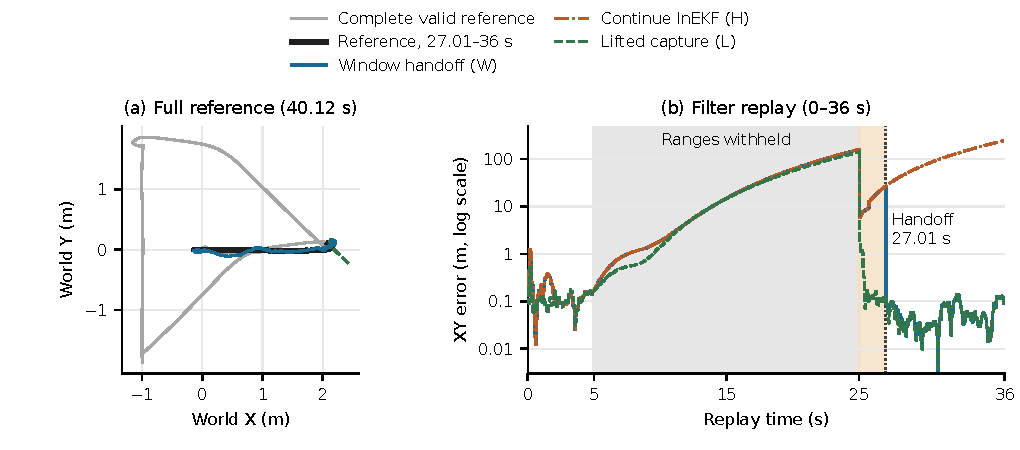
\includegraphics[width=\textwidth]{flight_trajectory.pdf}
\caption{Delft triangle, first in the fixed six-flight protocol. Left, the full valid motion-capture path spans 40.12 s. The highlighted reference and continuous handoff and lifted-capture estimates cover 27.01--36 s on equal spatial axes. Right, horizontal error for all three policies using the latest state at 20 Hz over \([0,36)\) s. Ranges were withheld over \([5,25)\) s. The first return arrived at 25.01 s and handoff followed at 27.01 s.}
\label{fig:trajectory}
\end{figure*}

On the triangle flight, the continued and handoff filters follow the same drifting state until the window is ready. The handoff then returns the estimate to the measured path (Fig.~\ref{fig:trajectory}). Over \([31,36)\) s, the handoff and lifted-capture filters both track it to 0.075 m horizontal RMSE. This score uses the latest emitted state at each scoring instant. The window fits in Fig.~\ref{fig:endpoints} contribute one position error per endpoint.

Across the six flights, a handoff after the 20 s outage reduces every late error (Table~\ref{tab:loop}). The median of the paired changes is \(-39.352\) m. In the 2--5 s interval the cohort median falls from 16.451 to 0.109 m. By 6--11 s it reaches the 0.092 m median of lifted capture. Continued filtering remains competitive after short indoor gaps.

The outdoor trial tests the same intervention across sites. After a 20\,s gap the two late cohort medians are 0.577 and 0.533 m, with a median within-recording change of \(+0.00056\) m. At 2\,s, continuing the filter gives the lower late error on six of eight supported recordings. These paired results favor using the outdoor window first as a position fix.

\subsection{Physical heading with the original TDoA InEKF}
For the original filter of Oursland and Mehrabian~\cite{oursland}, the published antenna offset \(\ell\) enters the ideal signed observation for anchors \(a,b\) as
\begin{equation}
 h_{ab}(R,p)=\norm{p+R\ell-b}-\norm{p+R\ell-a}. \label{eq:tdoa}
\end{equation}
This observation can change instantaneously with orientation through the lever arm. In the zero-lever-arm TWR model \eqref{eq:observation}, heading affects distances through the trajectory history. We therefore assess physical yaw with the original InEKF class on Toronto UTIL flights with motion-capture attitude~\cite{util}. Each cohort comprises four recordings and two initial-yaw interventions (\(0^\circ\) and \(180^\circ\)). The original event queue and covariance are retained. We suppress TDoA for \([10,20)\) s and score wrapped yaw and XY on \([26,45)\) s.

Reserving packets for an early XY update changes median horizontal/yaw RMSE from \(0.112\) m/\(5.93^\circ\) to \(0.087\) m/\(6.80^\circ\) in the primary cohort, and from \(0.0705\) m/\(7.22^\circ\) to \(0.0709\) m/\(6.22^\circ\) in the complementary cohort. The position and heading scores move independently even with genuine attitude truth. A component-wise decision at handoff is therefore consistent both with the measurement geometry in \eqref{eq:tdoa} and with the flight results.

\section{Discussion and conclusion}\label{sec:conclusion}
The window recovers position by combining two complementary descriptions of motion. The IMU records turns that a low-order range-only polynomial smooths away. Three acceleration-correction coefficients let that inertial shape adapt as integration error grows. Profiling yaw makes the combination practical with one nonlinear start. Across six indoor flights and ten outdoor recordings, the gain in horizontal endpoint accuracy is largest on the longest windows. With eight indoor anchors and the same range calibration, the 8\,s horizontal RMSE is 0.591 m for range-only quadratic reconstruction and 0.113 m for the proposed method. The rotating-bias derivation explains why a free quadratic also works well on short segments and how turning separates the two models.

The smaller projected singular value bounds seed sensitivity before fitting. The conditional curvature then measures the yaw information retained after refitting position, velocity and bias.

The acquisition equations require no vehicle-specific dynamics and can initialize a single InEKF. In the long indoor outage case, relinearizing one interval from its checkpoint restored the accuracy of an established capture method. The next step is to validate a component-wise handoff at a held-out site with synchronized antenna, prism and heading references. Measuring delivery latency on the flight processor and testing heading acceptance against those references would extend the present position result to a deployable recovery policy.

\begin{samepage}
\section*{Acknowledgment}
OpenAI Codex assisted with drafting and editing Sections I--VIII, checking derivations, and preparing plotting code for the analytic and flight-level figures from the recorded results. DeepSeek was used to cross-check descriptive arithmetic.
\par\end{samepage}

% Keep TAES name and continuation indents while easing stretched words in narrow columns.
\begingroup
\let\taesbibliography\thebibliography
\renewcommand{\thebibliography}[1]{%
  \taesbibliography{#1}\rightskip=0pt plus 2em\relax
  % The distributed bibliography resets \newblock before its first item.
  % Keep each short author, title, and publication entry together across columns.
  \interlinepenalty=10000\relax
  \let\taesbibitem\bibitem
  \def\bibitem{\def\newblock{\par\nobreak}\taesbibitem}}
% Use the class's reference break to balance the final two columns.
\IEEEtriggeratref{16}
\bibliographystyle{IEEEtaes}
\bibliography{references}
\endgroup
\end{document}
